\chapter{Capacitively Coupled Pixel Detectors for the CLIC Vertex Detector}
\label{chap:theory}

\chapterquote{There, sir! that is the perfection of vessels!}
{Jules Verne, 1828--1905}

\section{Introduction}
Successful identification of heavy-flavour quarks and tau-leptons relies upon precise reconstruction of the secondary displaced vertices produced in the decay of these particles as well as accurate association of the daughter tracks to those vertices.  To achieve this for the CLIC experiment very high spatial resolution, of approximately 3 {\mu}m and good geometric coverage extending to low $\theta$ values are essential.  The vertex detector must also have a low material budget, less than 0.2 $\text{X}_{0}$ per layer, as to not impact the performance of the other sub detectors and a low occupancy, aided by time-tagging to an accuracy of 10 ns, to counteract the high beam-induced backgrounds found near the impact point.  

There are no commercially available technology options that fulfil all the criteria for the vertex detector, which had led the CLIC experiment to consider a variety of new technology options.  The focus of this chapter is the use of high voltage complementary metal-oxide-semiconductor (HV-CMOS) active sensors coupled to a separate readout ASIC for the CLIC vertex detector.  

% Active sensor does something to signal when recorded, passive just records signel.  HV-CMOS is active as there's an amplification of signal step.

\subsection{HV-CMOS}
There are two classifications for pixel detectors; hybrid detectors where a passive sensor is bump-bonded to a separate readout chip and fully integrated where the collection diode is built upon the same wafer as the readout circuitry.  Both of these technology options find the CLIC experimental conditions extremely challenging.  Hybrid technologies struggle to achieved both the radiation tolerance and the functionality in the readout circuitry, while fully integrated circuits have too slow readout times due to limitations on the applied bias voltage.  

HV-CMOS is adapted to the CLIC experimental conditions as the n-MOS and p-MOS transistors forming the integrated amplifier (or generic in-pixel logic operations in general) for collecting the signal are embedded within a deep n-well, as shown in figure \ref{fig:hvcmos}.  This acts as both the collection diode as well as providing shielding to the circuitry from the beam induced radiation.  With the integrated circuitry shielded from the p-substrate it becomes possible to apply a large bias voltage to the substrate to widen the depletion region meaning that the main part of any signal deposited in the detector will be transferred via drift as opposed to diffusion, which provides the fast readout times required by the CLIC experiment.  

\begin{figure}
\centering
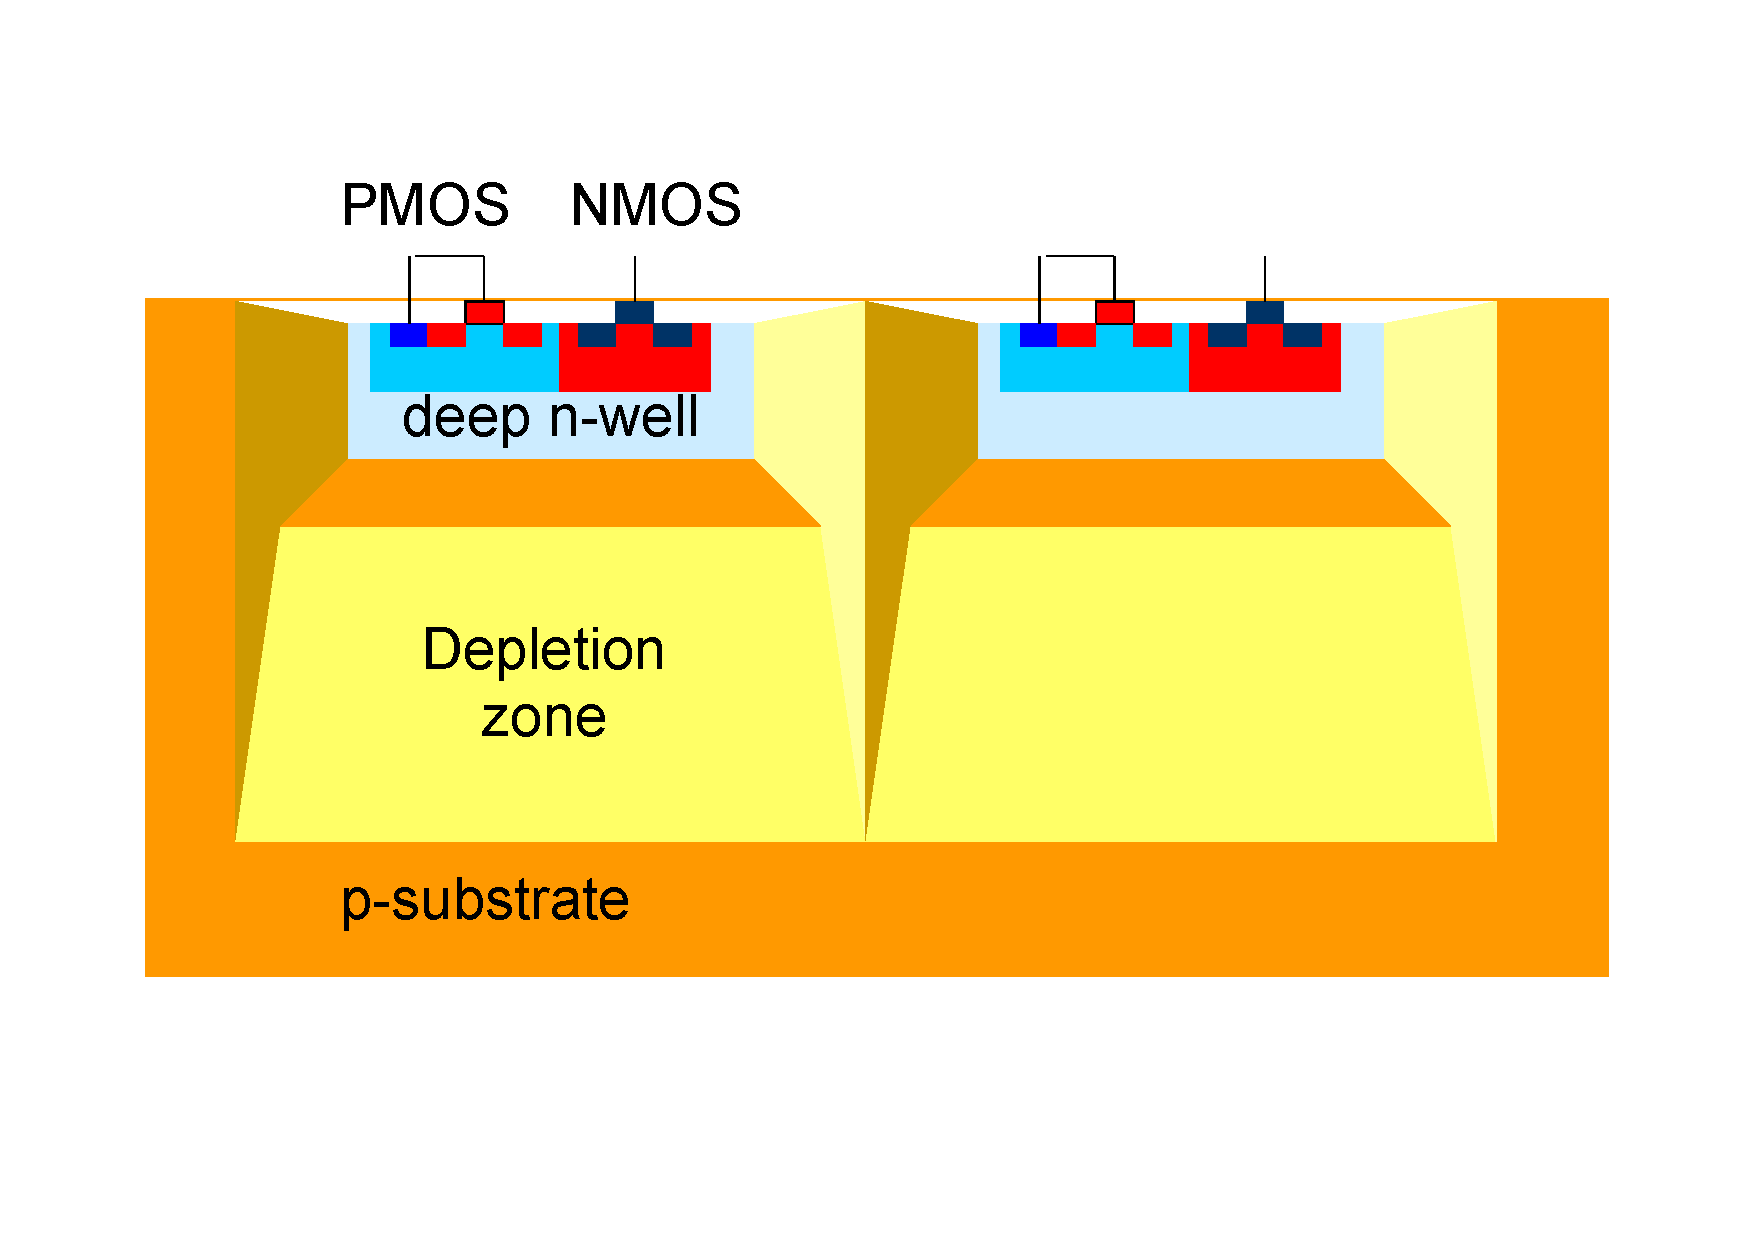
\includegraphics[width=0.5\textwidth]{CLICdpVertex/Plots/HV-CMOSDiagram.pdf}
\caption[HV-CMOS diagram.]{HV-CMOS diagram.}
\label{fig:hvcmos}
\end{figure}

HV-CMOS devices are strong candidates for the CLIC vertex detector, however, they do have limitations such as noise from interference between the n and p doped wells of the n-MOS and p-MOS transistors that sit within the deep n well.  This noise will grow with the number of n-MOS and p-MOS devices on the wafer and so ultimately restricts the complexity of the in-pixel operations that can be performed.  There are also topological difficulties such as the difficulty of applying the CMOS process to all sizes and the fact that the deep n well does not occupy the full space of the pixel.  

To minimise the material budget for the vertex detector, the pixels used are designed to be as thin as possible.  This means the signal from the HV-CMOS will be small as the depletion region will be thin.  To counter this, in-pixel signal amplification was applied to the HV-CMOS devices, as shown in figure \ref{fig:ccpdandclicpix}.  This increases the signal going to the readout ASIC, which also counteracts the intrinsically small capacitance between the HV-CMOS and readout ASIC.

\begin{figure}
\centering
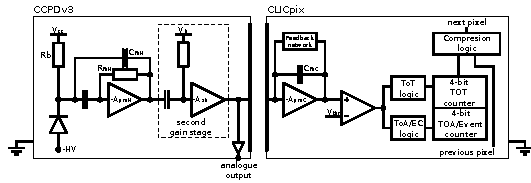
\includegraphics[width=0.5\textwidth]{CLICdpVertex/Plots/schematic.pdf}
\caption[Schematic of CCPDv3 and CLICpix pixels.]{Schematic of CCPDv3 and CLICpix pixels.}
\label{fig:ccpdandclicpix}
\end{figure}

\subsection{CLICpix}
The readout ASIC in this study is the CLICpix, which is a charge integrating amplifier connected to a discriminator as shown in figure \ref{fig:ccpdandclicpix}.  The output to this discriminator is then used as the input for further logic operations that record the magnitude, using a Time over Threshold (ToT) measurement, and time of arrival of the collected charge.

\subsection{Capacitive Coupling}
Solder bump-bonding is the typical method that is used for connecting active pixel sensors to the readout ASIC, however, the solder adds to the thickness of the sensor significantly as well as raising the cost.  A viable alternative to this procedure is the replacement of the bump-bonding with a thin uniform layer of glue that forms a capacitive connection between the active pixel and readout ASIC.  The mechanical tolerances on the alignment of the active pixel sensor and readout ASIC when applying this glueing procedure are the focus of this study.  

\section{Construction}
While replacing solder bump-bonding with a thin layer of glue in the construction of the sensors for the vertex detector offers benefits, such as reductions in the material budget and cost, the manufacturing procedure could lead to misalignments between the active pixel sensor and the readout ASIC.  To determine the impact of these misalignments a number of sensors were constructed using the gluing procedure that contained offsets between the HV-CMOS and CLICpix, as shown in figure \ref{fig:alignment}.  A table \ref{table:alignment} contains a summary of all the samples used in this study.

\begin{figure}
\centering
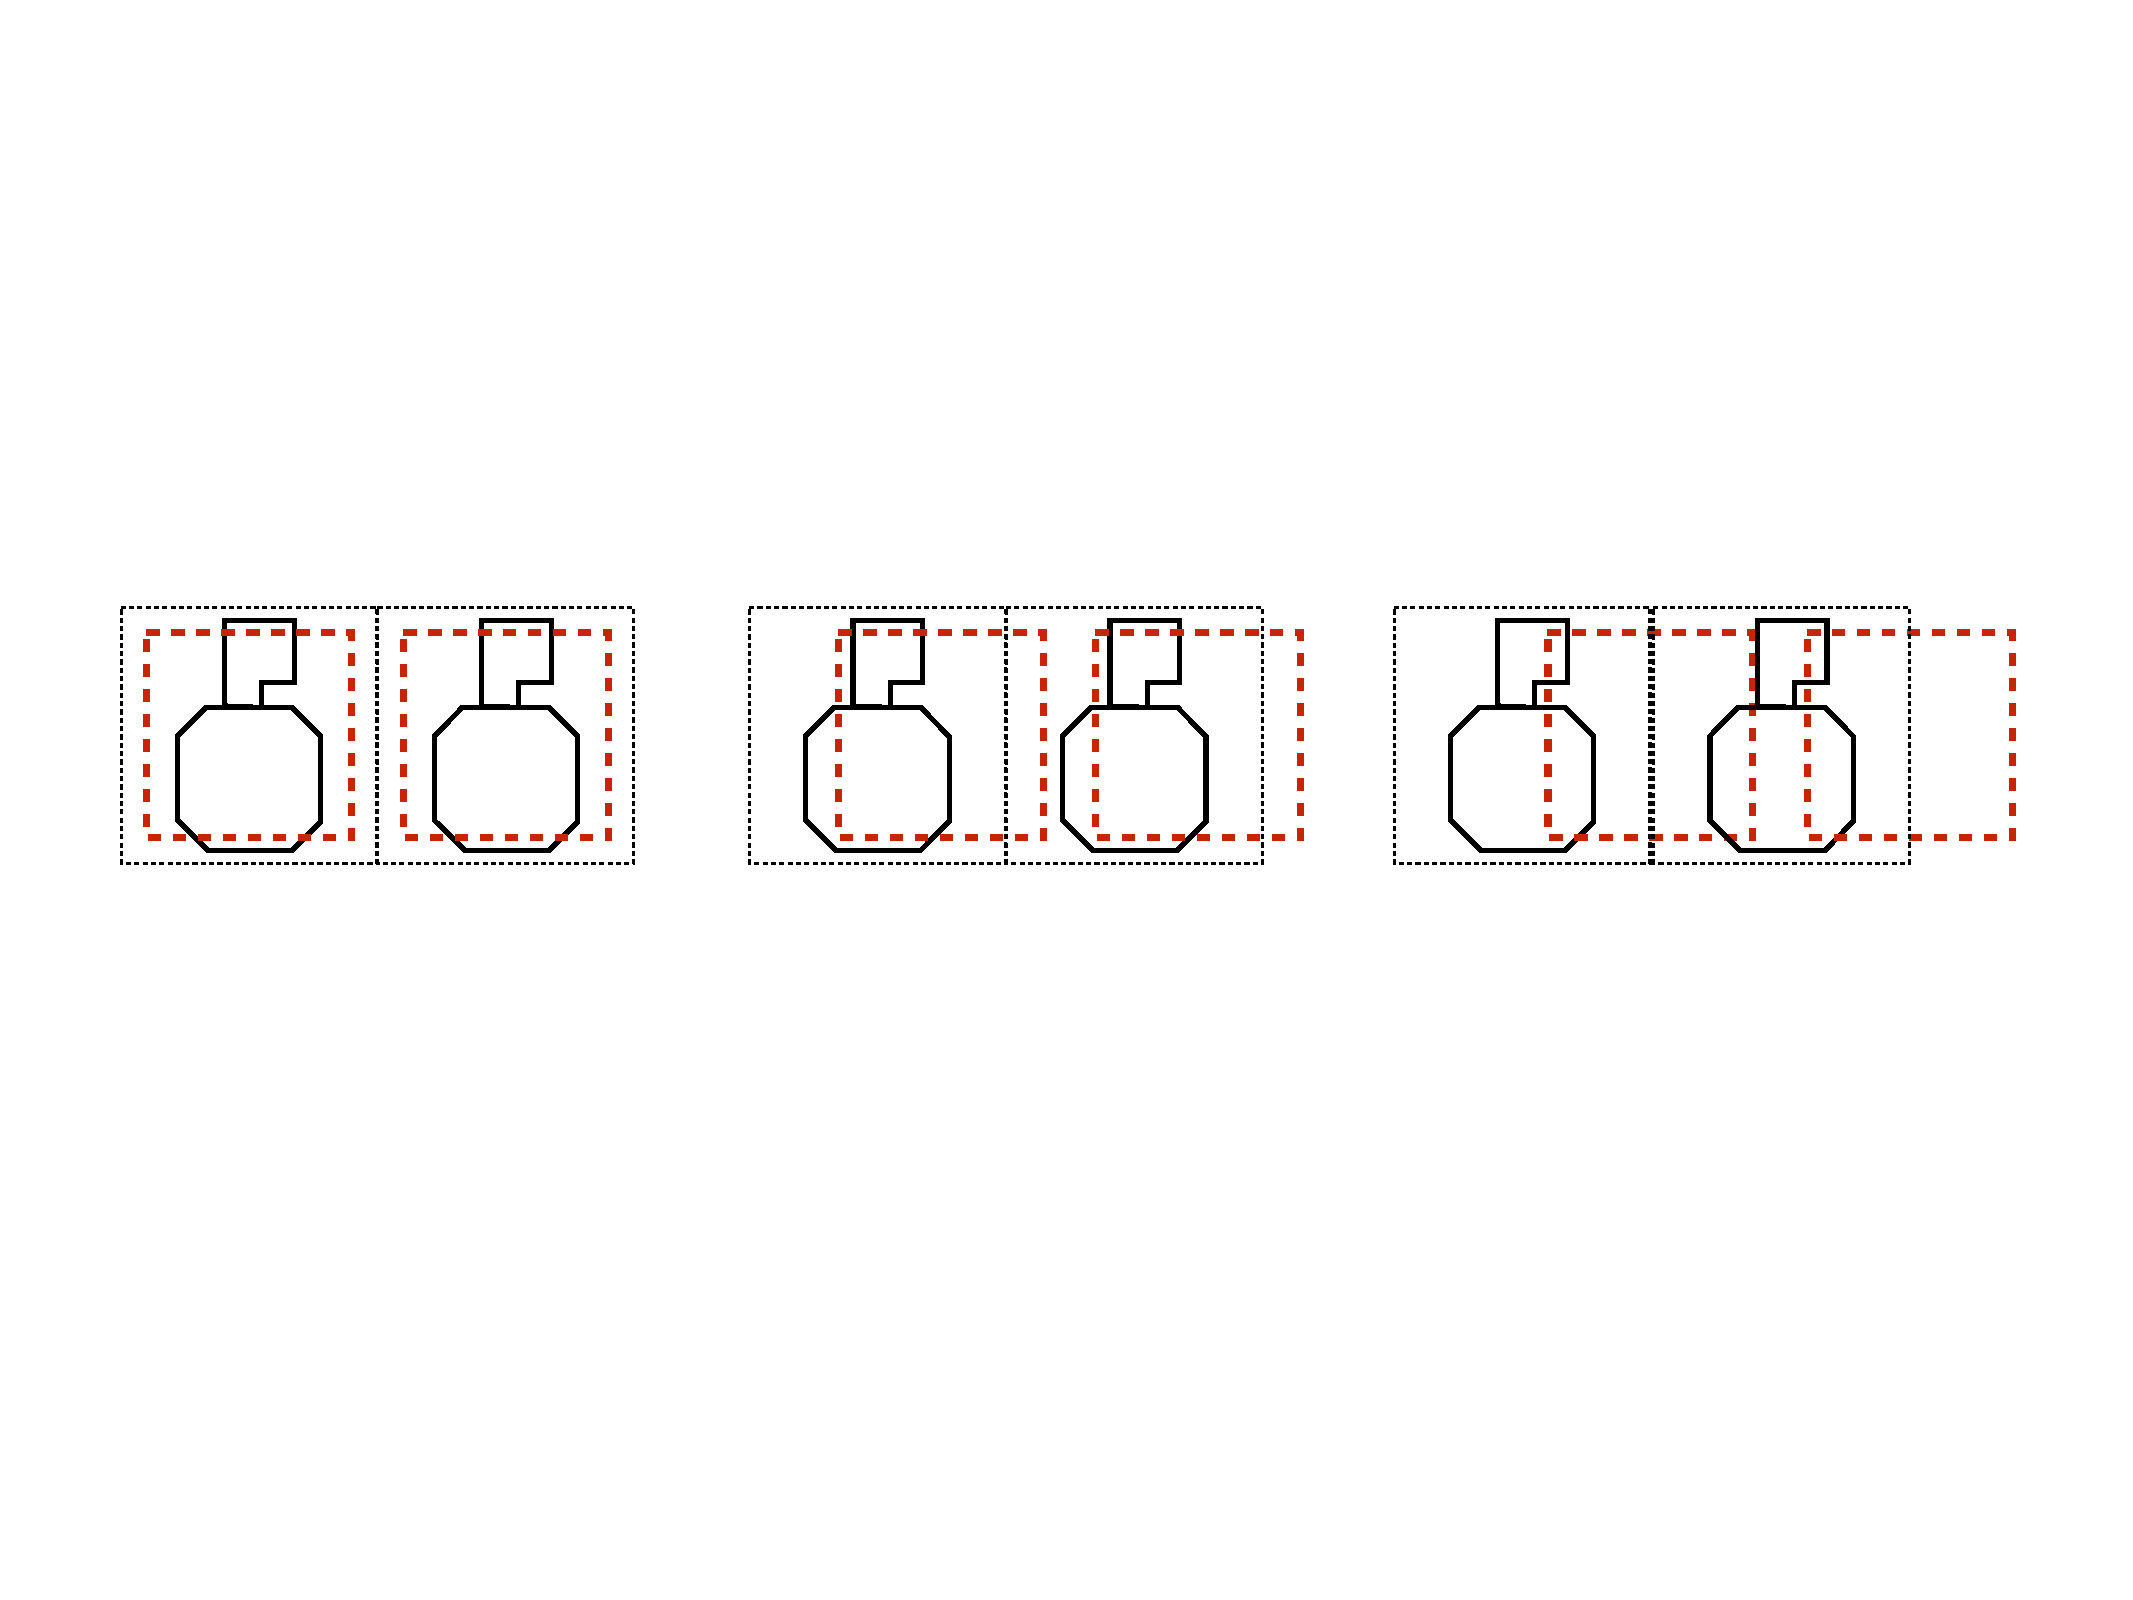
\includegraphics[width=1.0\textwidth]{CLICdpVertex/Plots/misalignedPads.pdf}
\caption[Schematic of alignment of CCPDv3 and CLICpix sensors studied in this analysis.]{Schematic of alignment of CCPDv3 and CLICpix sensors studied in this analysis.  The red dotted line represents the CCPDv3 and the solid black line represents the CLICpix.  From left to right; centred pixels, 1/4 offset (6.25 {\mu}m) and 1/2 offset (12.5 {\mu}m).}
\label{fig:alignment}
\end{figure}

\begin{table}[h!]
\centering
\begin{tabular}{ l l }
\hline
Assembly & Alignment \\ 
\hline
SET9 & Centred \\
SET10 & $\frac{1}{4}$ Offset \\
SET11 & $\frac{1}{2}$ Offset \\
SET12 & Centred \\
SET13 & Centred \\
SET14 & $\frac{1}{2}$ Offset \\
SET15 & Centred \\
SET16 & $\frac{1}{2}$ Offset \\
\hline
\end{tabular}
\caption[Description of alignment of sensors.]{Description of alignment of sensors.}
\label{table:alignment}
\end{table}

The pitch of the pixels produced was 25 {\mu}m and the matrix size was 64$\times$64.  The full details of the gluing process can be found here (CERN NOTE CITE) along with a study into the absolute precision of the manufacturing procedure.  It was found that for devices constructed in an identical fashion to those considered here, the glue layer thicknesses were less than 1 {\mu}m and the precision on the pixel positioning was less than 0.5 {\mu}m.  

\section{Device Characterisation}

This section describes the electrical tests that were performed on the sensor designed to determine the properties of the HV-CMOS and CLICpix.  

\subsection{CLICPix Calibration}
The first analysis was a radioactive source calibration.  This test involved using a strontium 90 

Compare the HV-CMOS pulse height to the ToT recorded on the CLICPix using strontium 90 sources.  Gives indication of gluing layer and CLICPix capacitances.  

\begin{itemize}
\item ToT vs pulse heights.  
\item ToT vs rise times.  
\end{itemize}

\begin{figure}
\centering
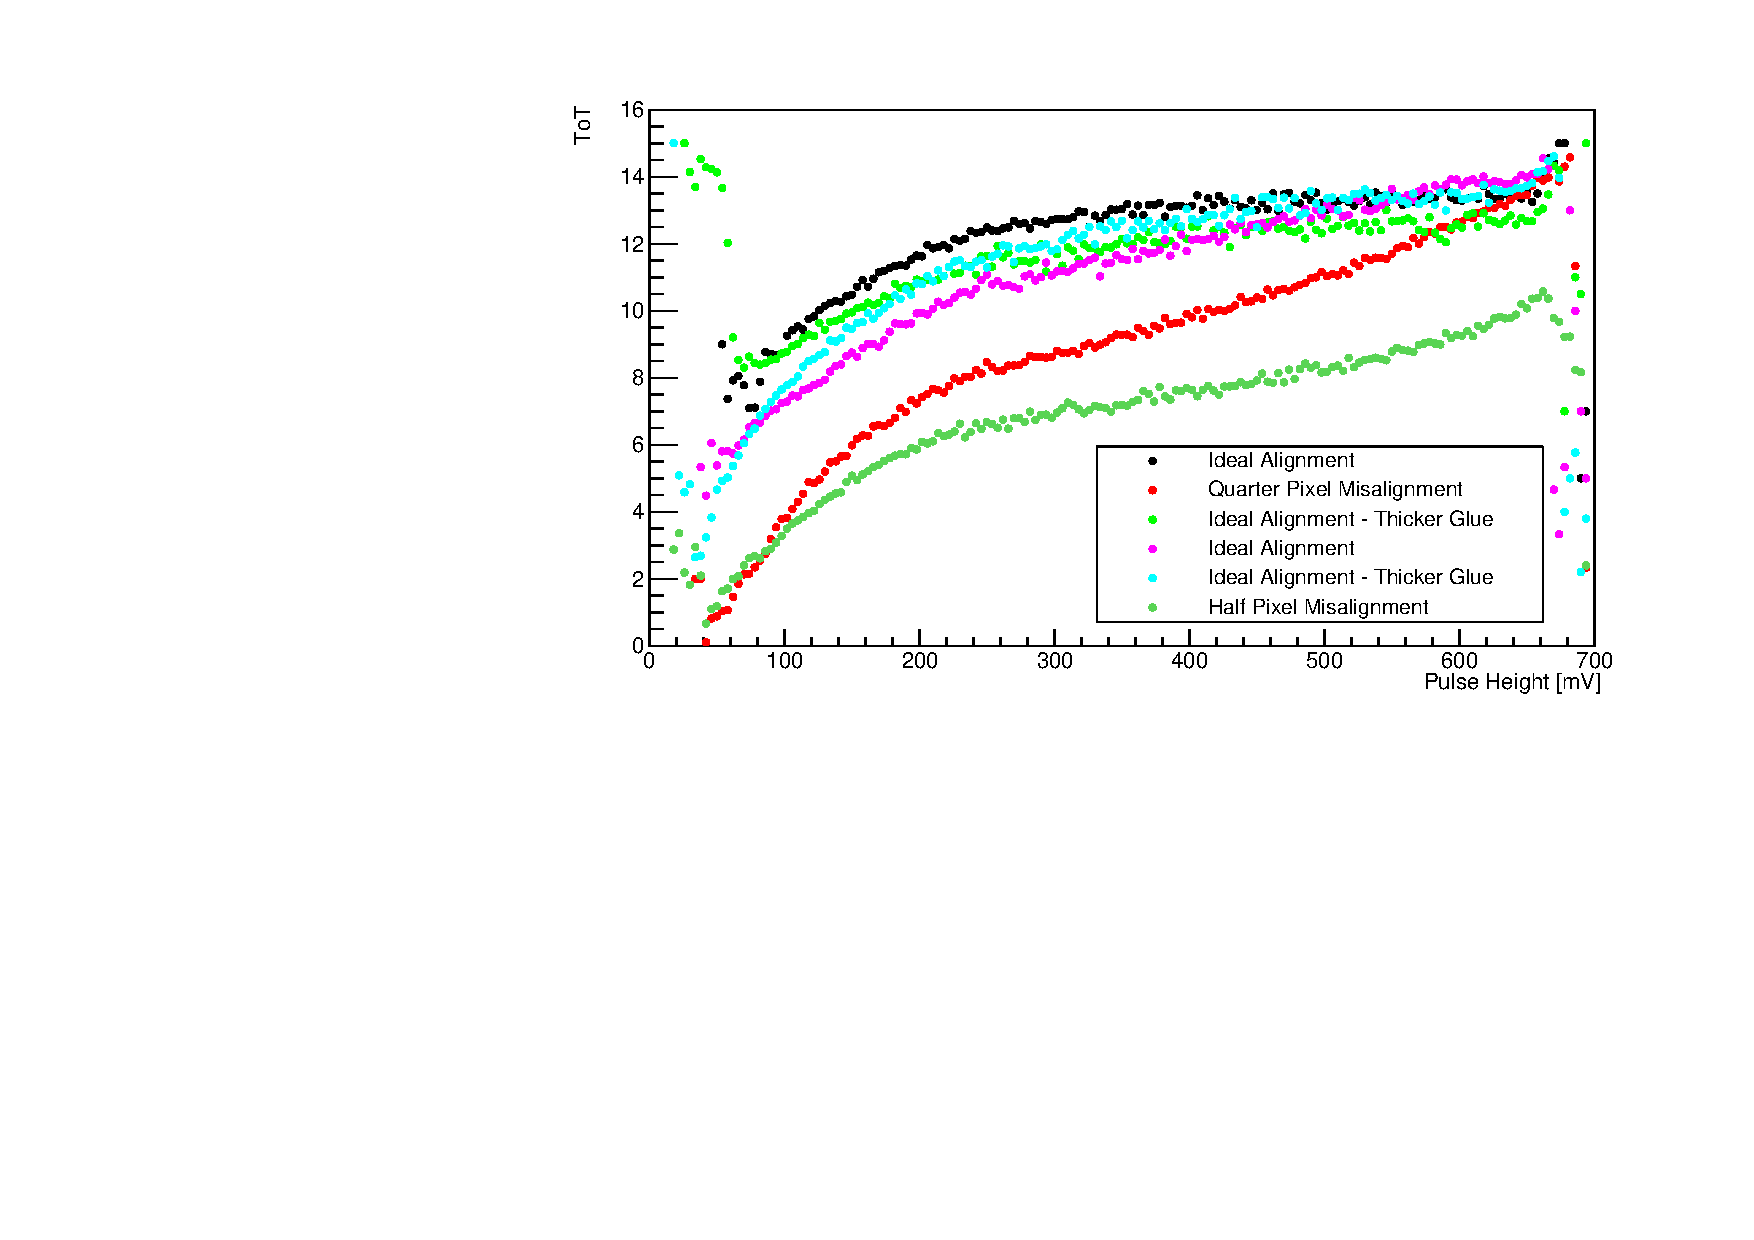
\includegraphics[width=0.5\textwidth]{CLICdpVertex/Plots/TargetToT_vs_PulseHeight.pdf}
\caption[Average ToT vs pulse height.]{Average ToT vs pulse height.}
\label{fig:avgtotvspulseheight}
\end{figure}

\begin{figure}
\centering
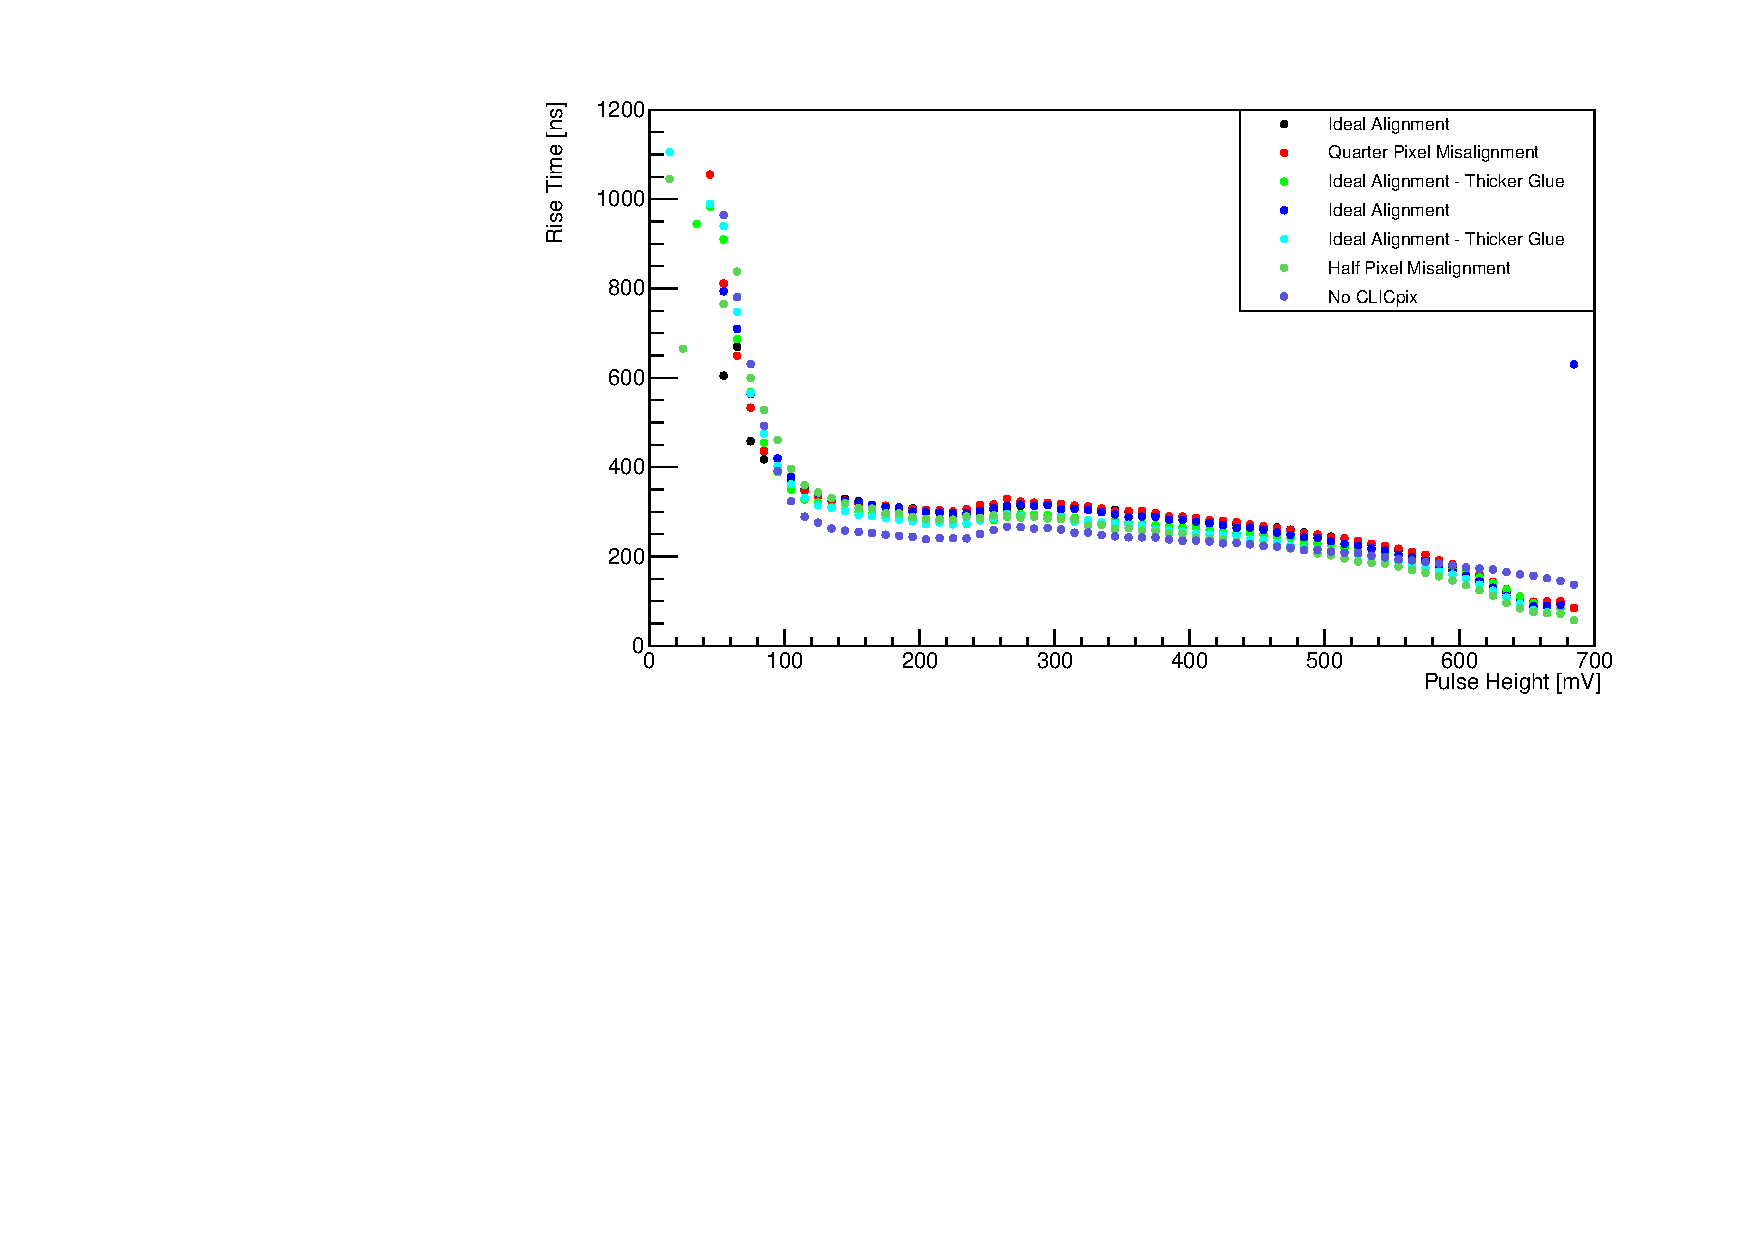
\includegraphics[width=0.5\textwidth]{CLICdpVertex/Plots/RiseTime_vs_PulseHeight.pdf}
\caption[Rise time vs pulse height.]{Rise time vs pulse height.}
\label{fig:risetimevspulseheight}
\end{figure}

\subsection{Cross Couplings}
ToT on adjacent cells vs pulse heights.  No charge sharing apparent except for SET16.  Possible issues with manufacturing other offset samples as some charge sharing is expcted.

\begin{figure}
\centering
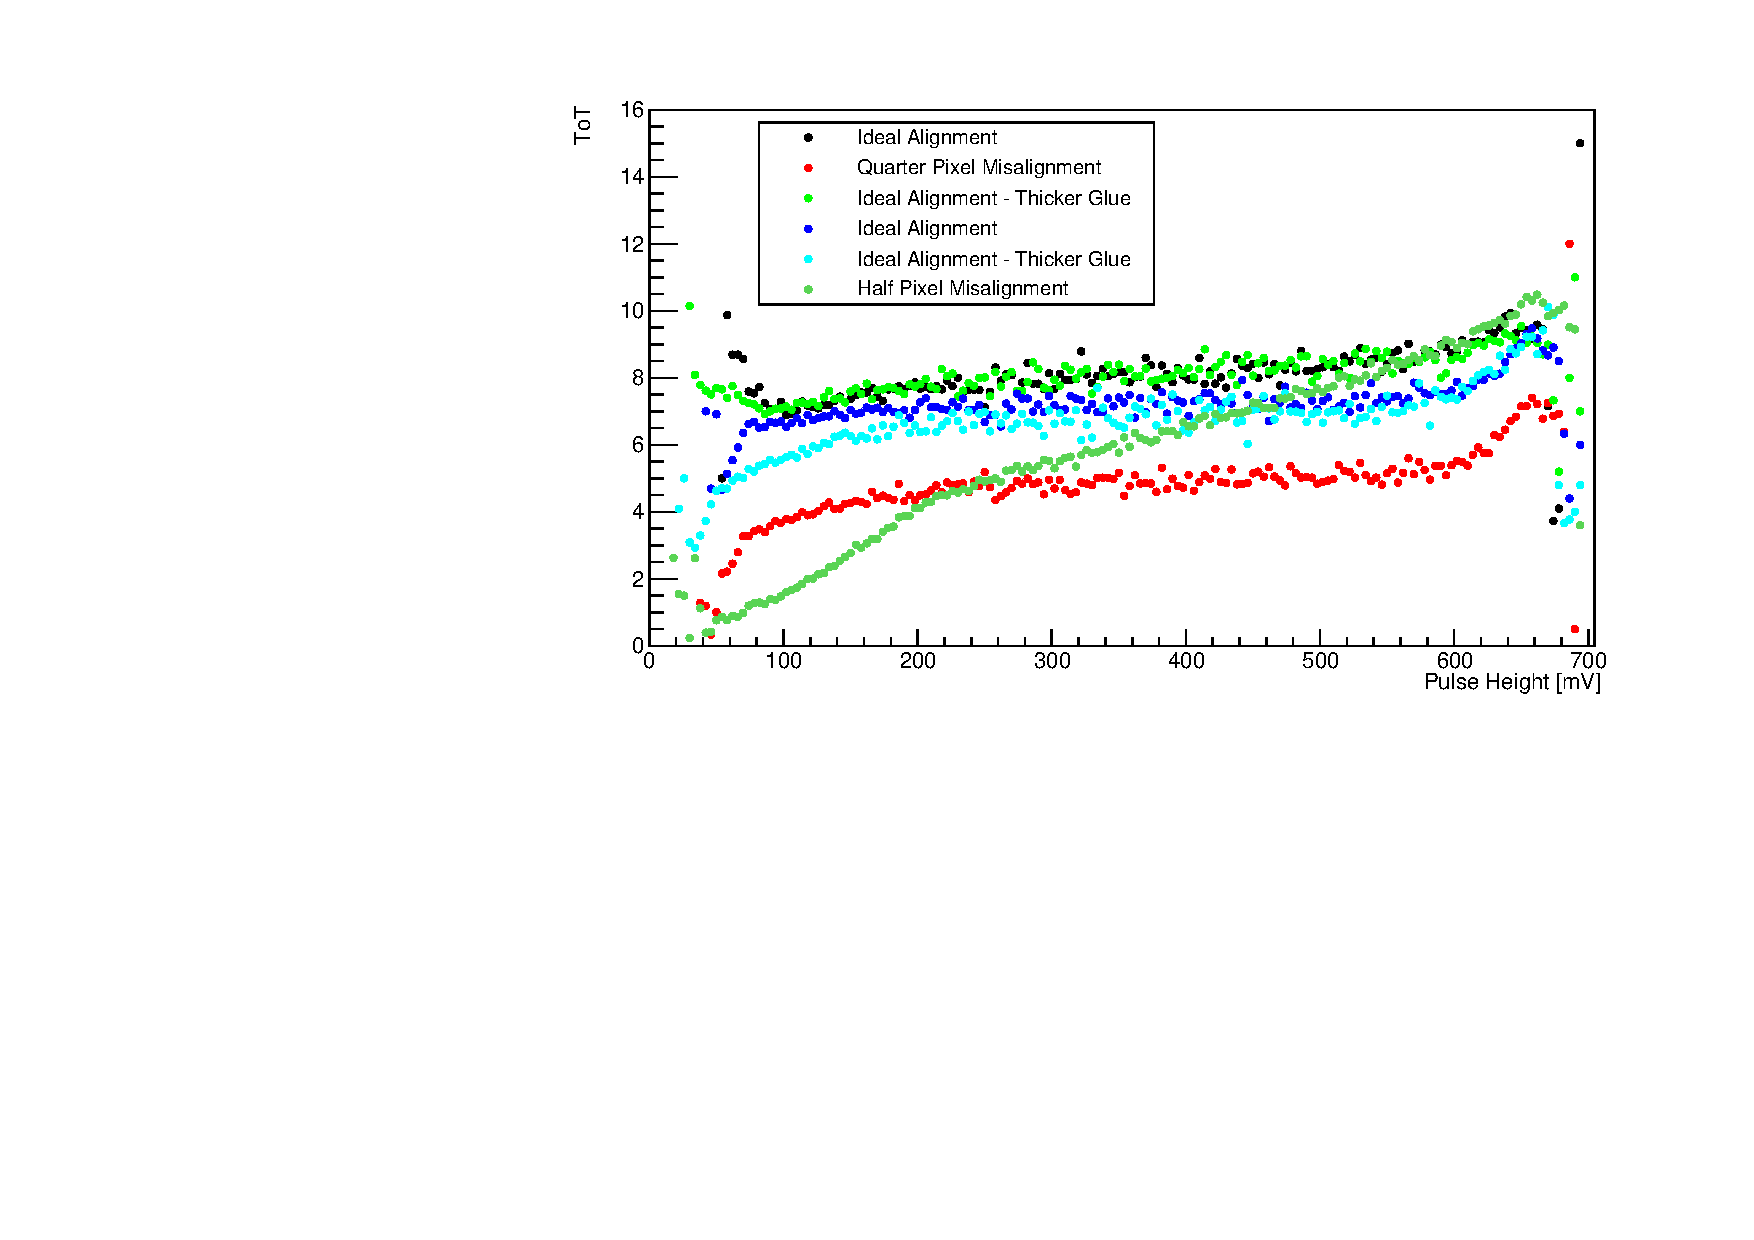
\includegraphics[width=0.5\textwidth]{CLICdpVertex/Plots/ToT_X_vs_PulseHeight.pdf}
\caption[Average ToT on adjacent pixel vs pulse height.]{Average ToT on adjacent pixel vs pulse height.}
\label{fig:avgtotadjvspulseheight}
\end{figure}

\subsection{Test Pulse Calibration}
Inject pulse height of fixed size directly into CLICPix and recored ToT.  This cannot be done for the HV-CMOS due to the device construction preventing getting to the relevant input to the HV-CMOS.  Plots of average ToT vs pulse height, describe surrogate function fit and column structure.  

\section{Test Beam Analysis}
\subsection{Test Beam Area}
Description of test beam, site and telescope.

\subsection{Efficiency}

\begin{itemize}
\item Description of masks and why they need to be applied.
\item Alignment description.
\item Efficiency calculations and conclusions. 
\end{itemize}

\begin{figure}
\centering
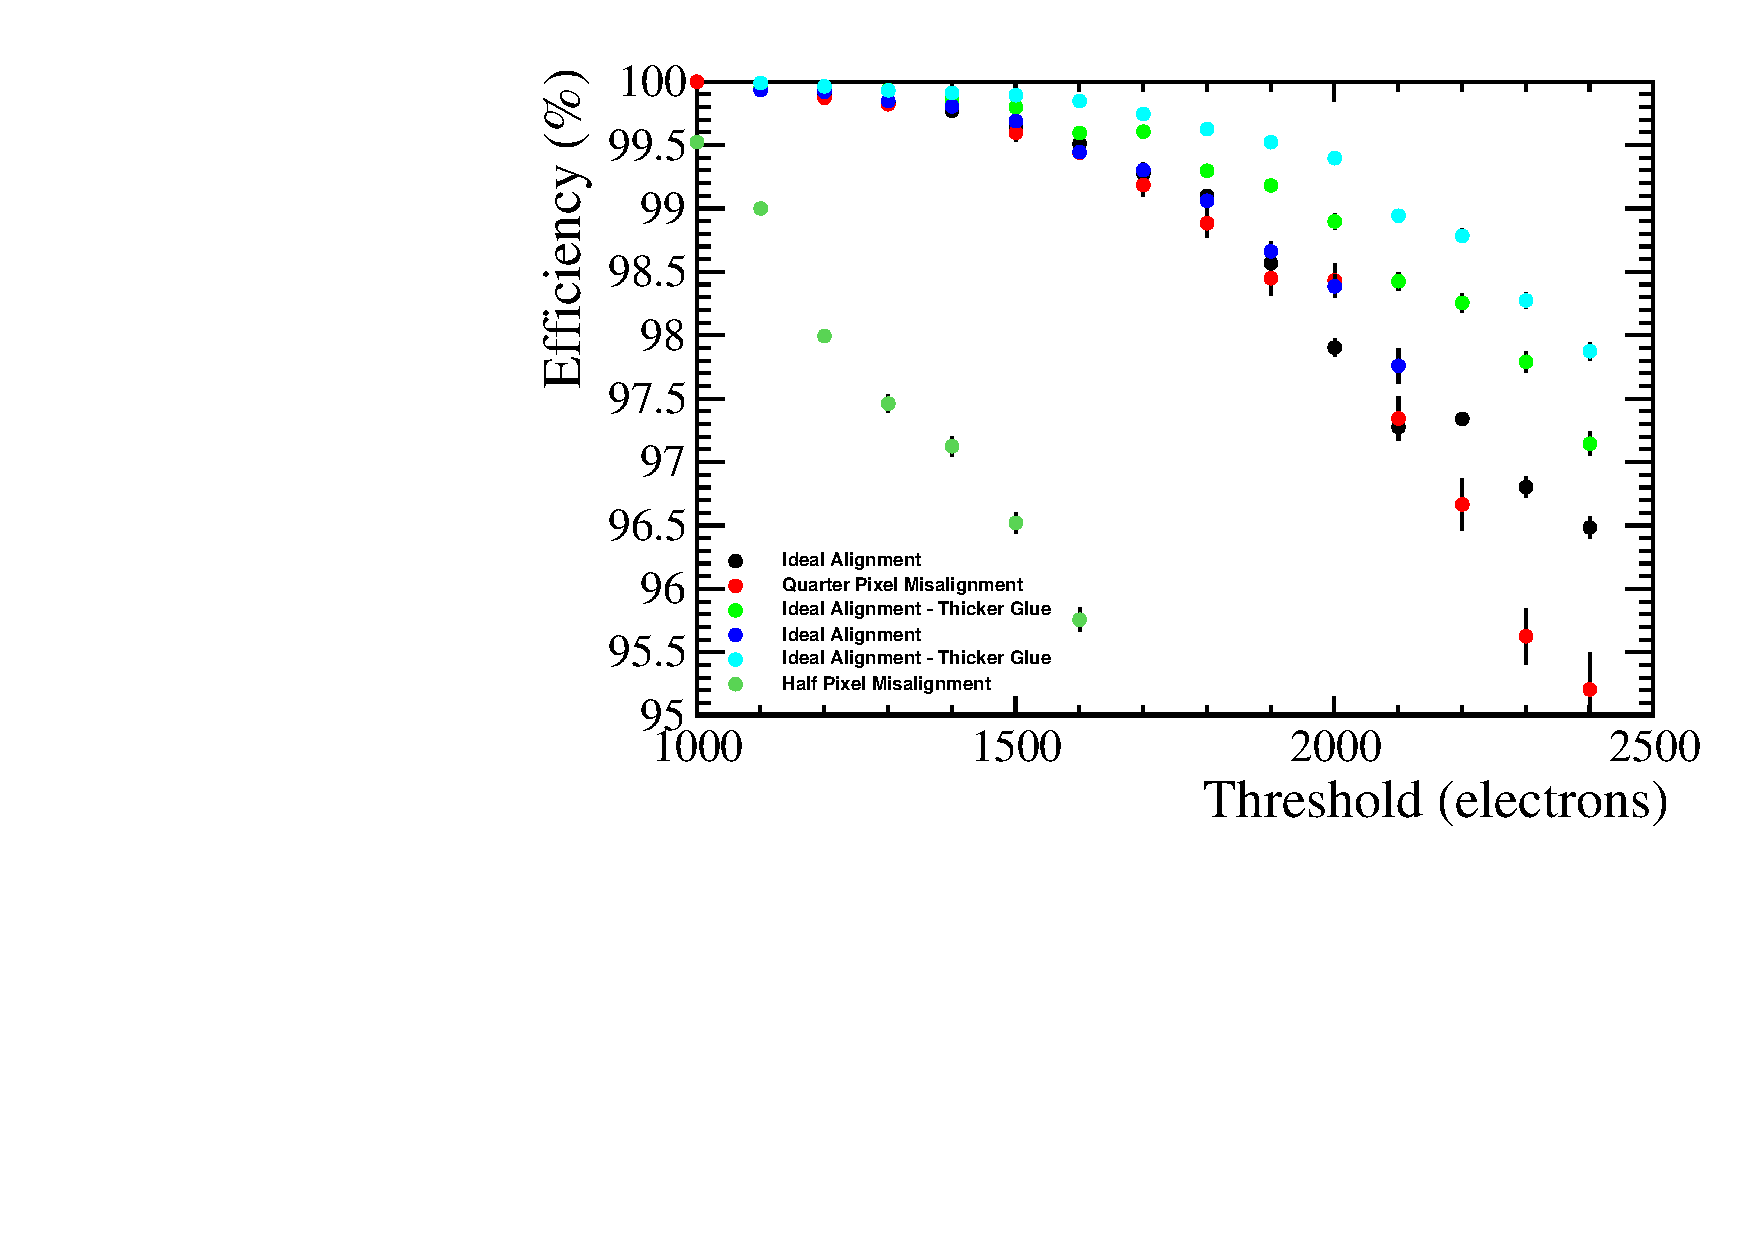
\includegraphics[width=0.5\textwidth]{CLICdpVertex/Plots/ZoomedEfficiency.pdf}
\caption[Efficiency vs threshold.]{Efficiency vs threshold.}
\label{fig:efficiency}
\end{figure}




  
